\documentclass[notes]{beamer}          % print frame + notes
%\documentclass[notes=only]{beamer}     % only notes
%\documentclass{beamer}                 % only frames
 
\usecolortheme{beaver}

% Some commonly used packages
% (copied mainly from the Utrecht University theme: https://www.overleaf.com/project/5c900fa3bd9930036341116a)
\usepackage{ragged2e}  % `\justifying` text
\usepackage{booktabs}  % Tables
\usepackage{tabularx}
\usepackage{tikz}      % Diagrams
\usetikzlibrary{calc, shapes, backgrounds}
\usepackage{amsmath, amssymb, amsfonts, amsthm}
\usepackage{url}       % `\url`s
\usepackage{listings}  % Code listings
\usepackage{comment}  
\usepackage{mathtools}
\usepackage{graphicx}
\usepackage{subfig}
\usepackage{amsmath}

% Mainly math commands
\newcommand{\vect}[1]{\bm{#1}}
\usepackage{amsfonts}% to get the \mathbb alphabet
\newcommand{\field}[1]{\mathbb{#1}}
\newcommand{\C}{\field{C}}
\newcommand{\R}{\field{R}}
\newcommand{\norm}[1]{\left\lVert#1\right\rVert}
\newcommand{\argmin}{\operatornamewithlimits{argmin}}
\providecommand{\abs}[1]{\lvert#1\rvert}
\providecommand{\norm}[1]{\lVert#1\rVert}

% A variable used to exclude slides from the lecture version
\newif\iffull
%\fullfalse
\fulltrue

% Bibliography 
\usepackage[uniquename=init,giveninits=true,maxcitenames=1,style=authortitle-comp,backend=bibtex8]{biblatex}
%\bibliography{references}
\addbibresource{references.bib}


%Information to be included in the title page:
\title{Classification: Support vector machines and random forests}
\author{Federica Eduati}
\institute{Eindhoven University of Technology

Department of Biomedical Engineering}
\date{2021}
 
 
\begin{document}
 
\frame{\titlepage}
 
\section{Overview}

\begin{frame}
\frametitle{Learning goals}
At the end of this lecture you will:
\begin{itemize}
    \item Have a general understanding of support vector machines for classification.
    \item Have a general understanding of machine learning methods based on decision trees (including random forests).
\end{itemize}

\vspace{5mm} 

Materials: 
\begin{itemize}
    \item Chapters 9, 12 and 15 from \cite{elements}
\end{itemize}

\end{frame}

\begin{frame}{Mentimeter}
Go to www.menti.com and use the code 47 08 97 17
\end{frame}



\section{General introduction}
\begin{frame}{Maximal margin classifier}

Classification problem: find a hyperplane that separates the classes in feature space.

\vspace{5mm} 

In $p$ dimensions a hyperplane is a flat affine subspace of dimension $p-1$, with general equation.

\begin{equation}
    f(x) = \beta_0 + \beta_1 X_1 + \beta_2 X_2 + \dots + \beta_p X_p = x^T\beta + \beta_0 = 0
\end{equation}

Where:
\begin{itemize}
    \item $\beta_0 = 0$ only if the hyperplane goes through the origin \item the vector $\beta = (\beta_1, \beta_2, \dots, \beta_p)$ is a unit vector ($\norm{\beta} = 1$) orthogonal to the surface of the hyperplane
\end{itemize}
    
\end{frame}


\begin{frame}{Maximal margin classifier}
Imagine to have a training data of N pairs: $\{(x_1, y_1), (x_2, y_2), \dots, (x_N, y_N)\}$, with $x_i \in {\rm I\!R}^p$ and $y_i \in \left\{-1,1 \right\}$.

If the classes are perfectly separable, there are generally multiple hyperplanes that can separate them.

\begin{center}
\includegraphics[height=5.5cm]{../figures/week_6/svm_hyperplanes.pdf}
\end{center}

\end{frame}


\begin{frame}{Maximal margin classifier}
The \textit{maximal margin classifier} is the one with biggest margin between the two classes.

\begin{center}
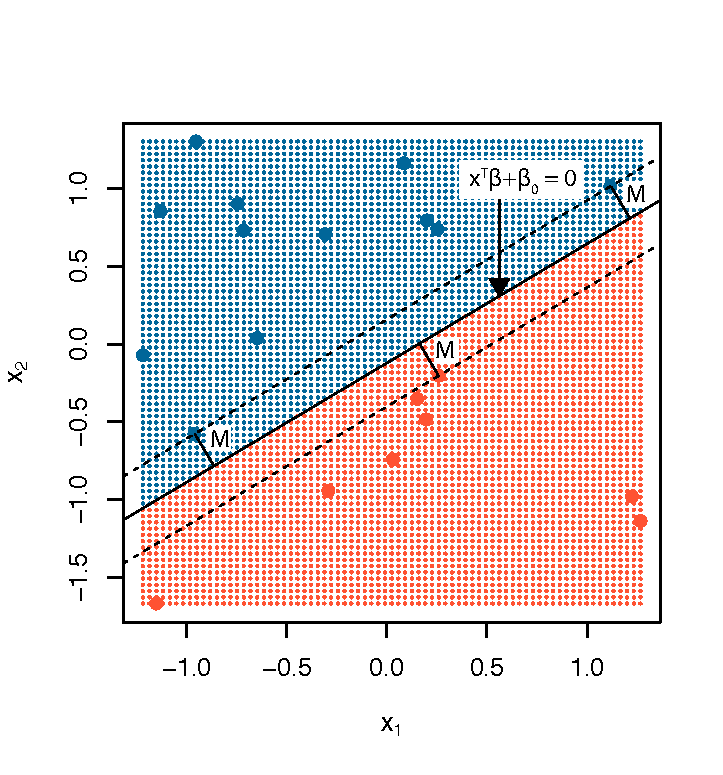
\includegraphics[height=5.5cm]{../figures/week_6/svm_maximal_margin_classifier.pdf}
\end{center}

\vspace{-7mm} 

\begin{equation*}
\max_{\beta, \beta_0, \norm{\beta} = 1} M \text{, subject to } y_i(x^T_i \beta + \beta_0) \geq M, i=1, \dots, N
\end{equation*}

\end{frame}

\begin{frame}{Noisy or non-separable data}
The maximal margin classifier has issues in case of:
\begin{itemize}
    \item Noisy data with outliers leading to poor solution (left panel - just added one data point to the previous example).
    \item Data non-separable by linear boundary (right panel).
\end{itemize}

\begin{center}
\includegraphics[height=5cm]{../figures/week_6/svm_outlier_or_not_separable.pdf}  
\end{center}
    
\end{frame}


\begin{frame}{Support vector classifier}

The \textit{support vector classifier} provides a solution by maximising a \textit{soft} margin (regularization).

\vspace{5mm}

For this we can modify the optimization problem allowing some slack.

\begin{equation*}
\max_{\beta, \beta_0, \norm{\beta} = 1} M \text{, subject to } y_i(x^T_i \beta + \beta_0) \geq M (1-\xi_i), i=1, \dots, N
\end{equation*}

where $\xi_i \geq 0$ and $\sum_{i=1}^N \xi_i \leq C$. $C$ is a constant that defines the budget we allow for the total amount of slack.

\vspace{5mm}



\end{frame}


\begin{frame}{Support vector classifier}

The \textit{support vector classifier} provides a solution by maximising a \textit{soft} margin.
\begin{center}
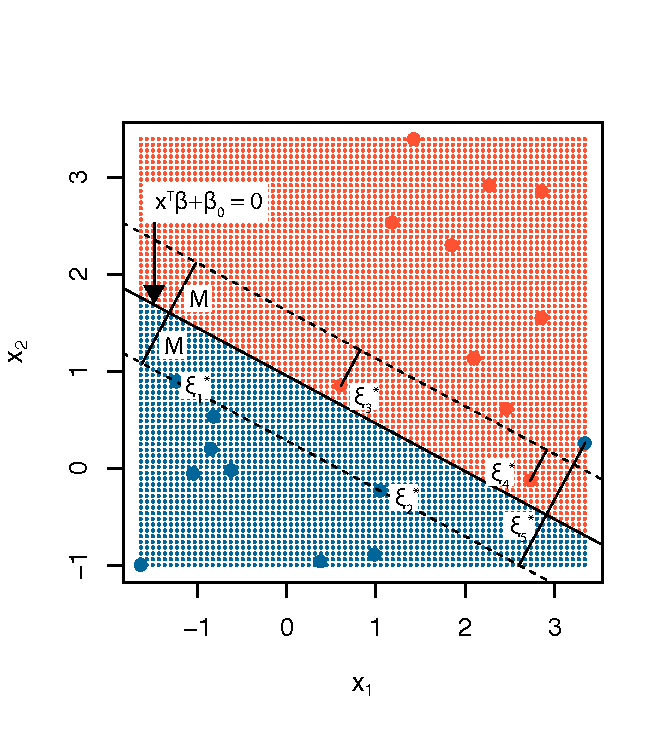
\includegraphics[height=5.5cm]{../figures/week_6/svm_support_vector_classifier.pdf}  
\end{center}

\vspace{-7mm} 

\begin{equation*}
\max_{\beta, \beta_0, \norm{\beta} = 1} M \text{, subject to } y_i(x^T_i \beta + \beta_0) \geq M (1-\xi_i), i=1, \dots, N
\end{equation*}

\end{frame}

\begin{frame}{Slack variables}

The slack variables $\xi = (\xi_1, \xi_2, \dots, \xi_N)$ tell us how much each point is allowed to be on the wrong side of its margin (relative amount).

\begin{itemize}
    \item $\xi = 0$ when the $i$th observation is on the correct side of the margin
    \item $\xi > 0$ when the $i$th observation is on the wrong side of the margin
    \item $\xi > 1$ when the $i$th observation is on the wrong side of the hyperplane
\end{itemize}


\end{frame}

\begin{frame}{Mentimeter question (www.menti.com code 47 08 97 17)}
How many points are on the wrong side of the hyperplane?
\begin{center}
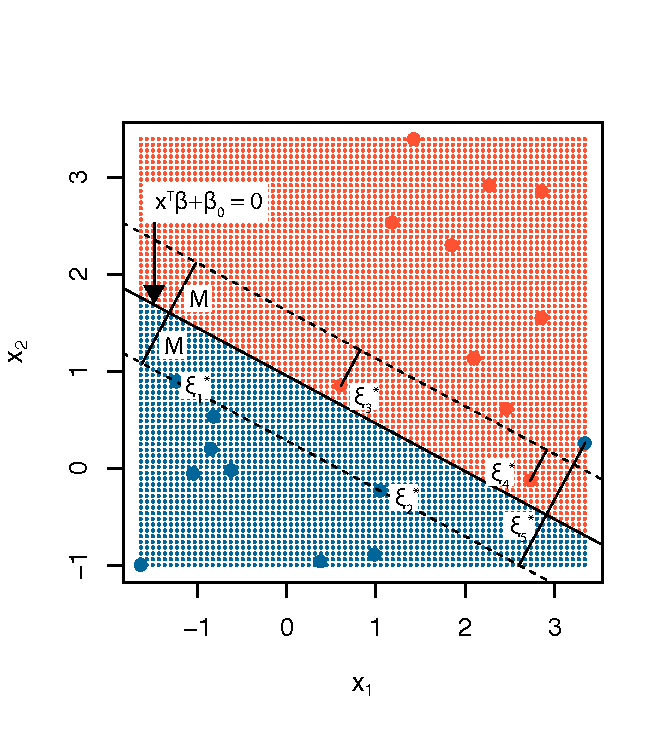
\includegraphics[height=5.5cm]{../figures/week_6/svm_support_vector_classifier.pdf}  
\end{center}
\end{frame}

\begin{frame}{Regularization}

The constant $C$ (slack budget) is tunable and can be seen as a regularization parameter.

\begin{itemize}
    \item $C = 0$ no budget for violation of the margin (maximum margin classifier)
    \item increasing $C$ allows more slack allowed (wider margins)
\end{itemize}

Therefore $C$\ controls the bias-variance trade-off:

\begin{itemize}
    \item small $C$ $\rightarrow$ narrow margins $\rightarrow$ high fit to the data $\rightarrow$ low bias, high variance
    \item large $C$ $\rightarrow$ wide margins $\rightarrow$ more violation allowed $\rightarrow$ high bias, low variance
\end{itemize}

\end{frame}

\begin{frame}{Example}

Example of support vector classifier for increasing values of $C$.

\begin{center}
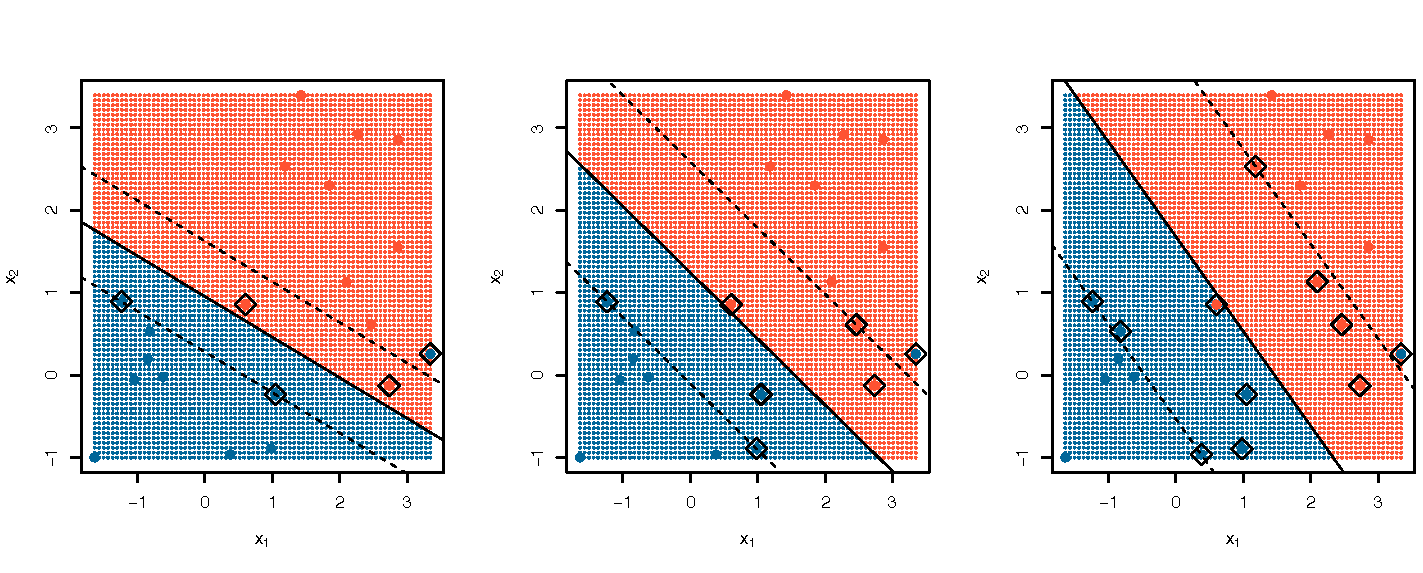
\includegraphics[height=4.2cm]{../figures/week_6/svm_support_vector_classifier_regularization_C.pdf}  
\end{center}

The \textit{support points} (marked with diamonds), i.e. those with $\xi_i \neq 0$, are the only ones that determine the orientation of the margin.

\end{frame}

\begin{frame}{Noisy and non-separable data}

The support vector classifier allows to have a good classifier in both the examples of noisy and non-separable data that we have seen earlier, where the maximal margin classifier was not working properly.

\begin{center}
\includegraphics[height=5cm]{../figures/week_6/svm_outlier_or_not_separable_support_vector_classifier.pdf}  
\end{center}

\end{frame}

\begin{frame}{Non-linearly separable classes}
\begin{center}
\includegraphics[height=6cm]{../figures/week_6/nonseparableclass.png}  
\end{center}


\end{frame}

\begin{frame}{Classification with non-linear decision boundaries}
Extension of the Support vector classifier to handle \textbf{non-linear class boundaries}. 
Idea: use of quadratic, cubic, and even higher-order polynomial functions of the predictors.
Example:
\begin{center}{
$X_1, X_2 \hspace{0.05\textwidth}\to\hspace{0.05\textwidth} X_1, X^2_1, X_2, X^2_2, X_1X_2$}
\end{center}
\begin{equation*}
	f(x)=\beta_0 + \beta_1X_1 + \beta_2X^2_1 + \beta_3X_2 + 		\beta_4Xˆ2X^2_2+ \beta_5X_1X_2 
\end{equation*}

Example with one dimension:
\begin{figure}
  \includegraphics[width=0.8\textwidth]{../figures/week_6/SVM_kernel}  
\end{figure}


\end{frame}


\begin{frame}{Support vector machines}

Problems:
\begin{itemize}
	\item Infeasible for high $p$
	\item Which polynomial order?
\end{itemize}
\vspace{0.5cm}
\textit{Support vector machines} (SVM): extension of the support vector classifier which enlarges the feature space by using \textbf{kernels}.\\
\vspace{0.5cm}
The kernel approach is an efficient computational methodology to enlarge the feature space.


\end{frame}

\begin{frame}{Support Vector Machines}
Inner product definition:$\langle {a,b} \rangle = \sum_{i=1}^{p} a_{i}b_{i},$ where a,b are vectors\\~\\
The solution to the support vector classifier problem involves only the inner products of the observations. The inner product of two observations $x_i, x_i'$ is given by
\begin{equation*}
\langle {x_i,x_i'} \rangle = \sum_{j=1}^{p} x_{ij} x_{ij}' 
\end{equation*}
Then, the linear support vector classifier can be represented as:
\begin{equation*}
f(x) = \beta_0 + \sum_{i=1}^{N} \hat \alpha_i \langle {x,x_i} \rangle
\end{equation*}
where there are \textit{N} parameters $\hat \alpha_i$, one per training observation.
\end{frame}

%


\begin{frame}{Support Vector Machines}
$\hat{\alpha}_i$ is nonzero only for the support vectors. \\~\\
So if $\mathit{S}$ is the collection of indices of these support points, we can rewrite f(x) which involves far fewer terms than before:
\begin{equation*}
f(x) = \beta_0 + \sum_{i\in\mathit{S}} \hat{\alpha}_i \langle {x,x_i} \rangle,
\end{equation*}
Abstraction of the inner product:
\begin{equation*}
\mathit{K}(x_i,x_i'),
\end{equation*}
where we refer to $\mathit{K}$ as \textit{kernel}. 
A \textit{kernel} is a function that quantifies the similarity of two observations.
\end{frame}

\begin{frame}{Mentimeter question (www.menti.com code 47 08 97 17)}
How many $\hat \alpha$ do we have to estimate in this case?
\begin{center}
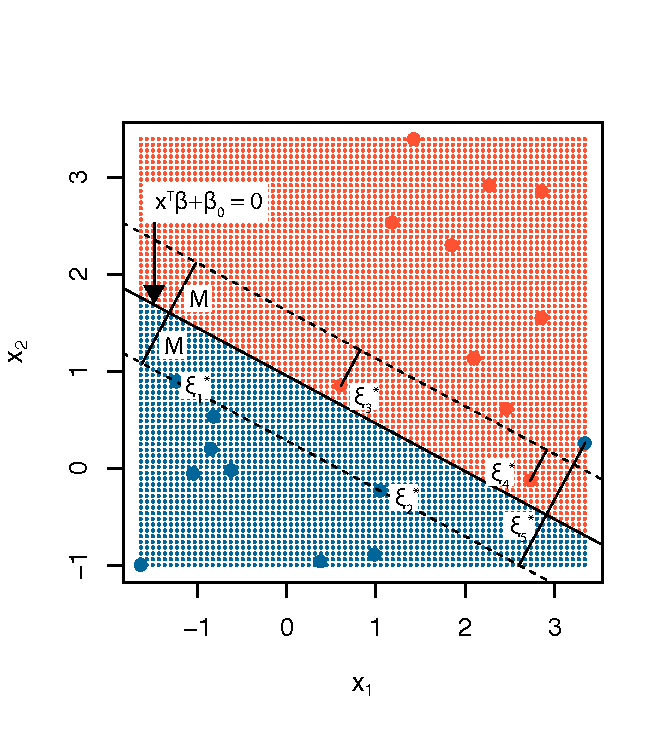
\includegraphics[height=5.5cm]{../figures/week_6/svm_support_vector_classifier.pdf}  
\end{center}
\end{frame}

\begin{frame}{Support Vector Machines}
Linear kernel: $\mathit{K}(x_i,x_i') = \sum_{j=1}^{p} x_{ij} x_{ij}' $ \\
Polynomial kernel of degree d: $\mathit{K}(x_i,x_i') = (1+ \sum_{j=1}^{p} x_{ij} x_{ij}')^d$\\
Radial kernel: $\mathit{K}(x_i,x_i') = exp(- \gamma \sum_{j=1}^{p} (x_{ij}-x_{ij}')^2)$ \\~\\
What is the advantage of using a kernel rather than simply enlarging the feature space using functions of the original features?
\begin{itemize}
 \item Computational advantage: we don't work in the enlarged feature space.
  \item Automatically computes inner product for high dimensional space of features.
  \item Avoid overfitting by automatically squashing down most dimensions.
\end{itemize}
\end{frame}

\begin{frame}{Extension to multi-class}
So far, binary classification, in other words, two-class setting. \\~\\
SVMs: concept of separating hyperplanes does not lend itself to more than two classes. \\~\\
Two approaches for extending SVMs to K$>$2 classes classification:
\begin{itemize}
 \item One-Versus-One Classification: $\binom{K}{2}$ SVMs comparing pair of classes. We assign the test observation to the class most frequently selected in these pairwise classification.
 \item One-Versus-All Classification: K SVMs, each time comparing one of the K classes to the remaining K-1 classes. We assign the test observation to the class (SVM in this case) with the best discrimination rule. 
\end{itemize}
\end{frame}

\section{Tree-based methods}
\begin{frame}{Tree-based methods}
\begin{itemize}
 \item Can be used for \textit{regression} or \textit{classification}
 \item Partition the feature space into a set of rectangles (consecutive binary partitions)
 \item This can be summarised into a tree: decision-trees
 \end{itemize}
 
 \begin{figure}
\minipage{0.22\textwidth}
  \includegraphics[width=\linewidth]{../figures/week_6/tree-example-a.pdf}  
\endminipage\hfill
\minipage{0.26\textwidth}
  \includegraphics[width=\linewidth]{../figures/week_6/tree-example-b.pdf}  
\endminipage\hfill
\minipage{0.46\textwidth}%
  \includegraphics[width=\linewidth]{../figures/week_6/tree-example-c.pdf}  
\endminipage
\end{figure}

\end{frame}



\begin{frame}{Example}
Coimbra Breast Cancer dataset

(Patricio, M., et al, BMC Cancer, 2018)
\vspace{-1cm}
\begin{center}
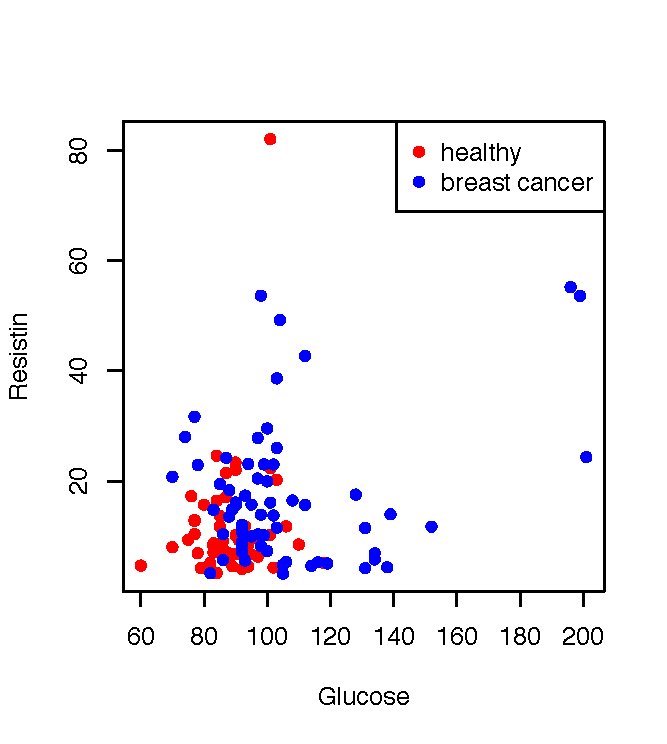
\includegraphics[height=8cm]{../figures/week_6/breast_cancer_2Dscatterplot.pdf}  
\end{center}
\end{frame}

\begin{frame}{Example}
 \begin{figure}
\minipage{0.5\textwidth}
  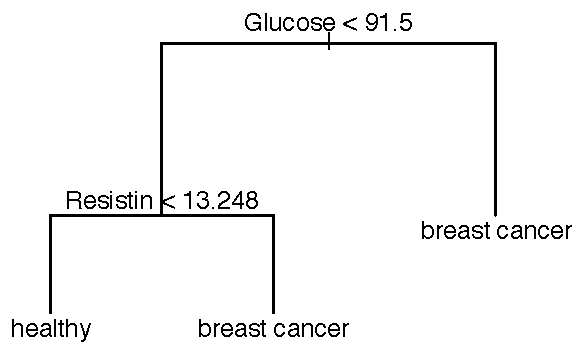
\includegraphics[width=\linewidth]{../figures/week_6/breast_cancer_tree.pdf}  
\endminipage\hfill
\minipage{0.5\textwidth}%
  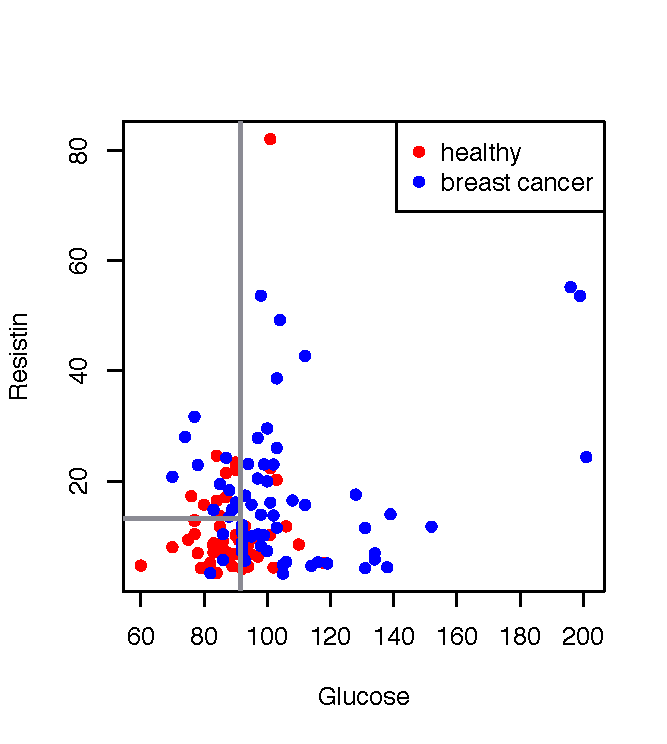
\includegraphics[width=\linewidth]{../figures/week_6/breast_cancer_2Dscatterplot_vhlines.pdf}  
\endminipage
\end{figure}
\end{frame}

\begin{frame}{Mentimeter question (www.menti.com code 47 08 97 17)}
For which ones the decision boundary was defined using a decision tree?
\begin{center}
\includegraphics[height=5cm]{../figures/week_6/Question_decision_tree}  
\end{center}
\end{frame}

\begin{frame}{Mentimeter question (www.menti.com code 47 08 97 17)}
Which scenarios are suitable for decision trees?
\begin{center}
\includegraphics[height=5cm]{../figures/week_6/Question_decision_tree}  
\end{center}
\end{frame}



\begin{frame}{How to build a decision-tree}
To grow a decision-tree we need a set of training data with $N$ observations consisting in $p$ inputs and a response
$(x_1,y_1) \dots (x_N,y_N)$, where each $x_i=(x_{i1}, x_{i2}, \dots, x_{ip})^T$ is a vector of feature measurements for the $i$th case.

\vspace{0.5cm}

The algorithm should build the decision tree that:

\begin{itemize}
\item divides the predictor space in $M$ non-overlapping regions $R_m$ with $m=1,...,M$ ($M$ number of leaves). For each observation that falls in the same region $R_m$ we make the same prediction.
\item this partition should minimise the $RSS$ (for regression) or the misclassification (for classification).
\end{itemize}
\end{frame}

\begin{frame}{How to build a decision-tree}
It is infeasible to evaluate every possible partition of the feature space.

\vspace{0.5cm}
We adopt an approach that is:
\begin{itemize}
	\item \textit{top-down}: starts from the top of the tree and proceeds with subsequent splits.
	\item \textit{greedy}: it looks at the optimal splitting at that specific step of the tree, without looking ahead. 
\end{itemize}
\end{frame}

\begin{frame}{How to build a decision-tree}
\begin{itemize}
	\item We start from the top of the tree and we select the variable $X_j$ and the splitting point $s$ to define the pair of half-planes $R_1(j,s)=\{X|X_j \le s\}$ and $R_2(j,s)=\{X|X_j > s\}$ that leads to the greatest reduction of the cost function.
	\item This will generate two nodes, for each of the node we repeat the procedure but looking only at the data in that half-plane. 
	\item This continue until we reach a termination criterion (e.g. no region with more than 5 observations).
\end{itemize}	

\end{frame}

\begin{frame}{Example}
 \begin{figure}
\minipage{0.5\textwidth}
  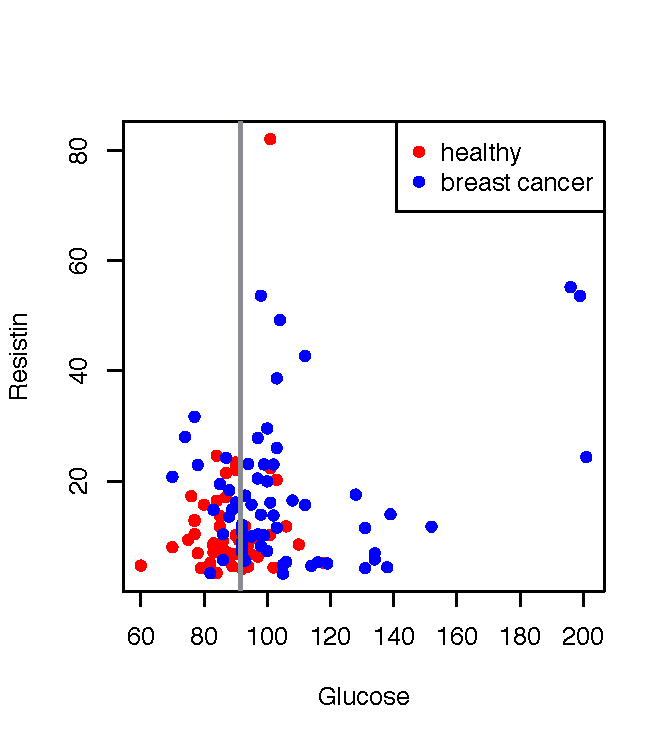
\includegraphics[width=\linewidth]{../figures/week_6/breast_cancer_2Dscatterplot_vline.pdf}  
\endminipage\hfill
\minipage{0.5\textwidth}%
  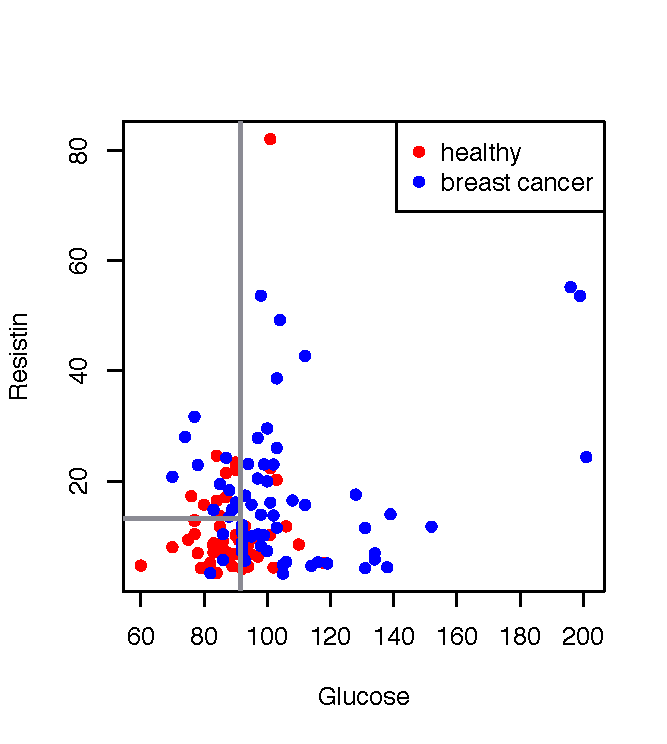
\includegraphics[width=\linewidth]{../figures/week_6/breast_cancer_2Dscatterplot_vhlines.pdf}  
\endminipage
\end{figure}
\end{frame}

\begin{frame}{Mentimeter question (www.menti.com code 47 08 97 17)}
What happens for a \textbf{regression tree} if there is no termination criterion?
\begin{itemize}
\item The tree goes to infinity
\item Each leaf has one observation only
\item It is not possible to tell without seeing the data
\end{itemize}	
\end{frame}

\begin{frame}{Mentimeter question (www.menti.com code 47 08 97 17)}
What happens for a \textbf{classification tree} if there is no termination criterion?
\begin{itemize}
\item The tree goes to infinity
\item Each leaf has one observation only
\item It is not possible to tell without seeing the data
\end{itemize}	
\end{frame}



\begin{frame}{Cost functions}
Let $N_m$ be the number of observations falling in region $R_m$.

For \textbf{regression}:
$$\dfrac{1}{N_m}\sum_{x_i\in R_m}(y_i-\hat c_m)^2  \quad \mbox{, where} \quad \hat c_m = \dfrac{1}{N_m}\sum_{x_i\in R_m}y_i$$
For \textbf{classification}:
\begin{equation*}
	\hat{p}_{mk}=\dfrac{1}{N_m}\sum_{x_i\in R_m}I(y_i=k)
\end{equation*}

is the proportion of training observations in region $m$ that are from class $k$. Different measures of node impurity include:
\begin{itemize}
\item  \textbf{Misclassification error}: $1-\max_k \hat{p}_{mk}$
\item  \textbf{Gini index}: $\sum_{k=1}^K\hat{p}_{mk}(1-\hat{p}_{mk})$
\item  \textbf{Cross-entropy or deviance} $-\sum_{k=1}^K\hat{p}_{mk}\log\hat{p}_{mk}$
\end{itemize}
\end{frame}


\begin{frame}{Predictions using a decision-tree}
What value will each leaf predict?
\begin{itemize}
	\item For \textbf{regression}: the average of the  training observations falling in the region $R_m$ of the leaf $m$.
		\item For \textbf{classification}: the most occurring class in the region $R_m$ of the leaf $m$.
\end{itemize}

\vspace{0.5cm}

\end{frame}

\begin{frame}{Mentimeter question (www.menti.com code 47 08 97 17)}
What is the risk of a tree with a lot of leaves?
\end{frame}

\begin{frame}{Pruning a tree}
Idea: build a large tree $T_0$ and then prune it back to a subtree $T$.

This is done defining a cost complexity criterion:
$$\sum_{m=1}^{|T|}\sum_{x_i\in R_m}(y_i-\hat c_m)^2+\alpha|T|$$

where:
\begin{itemize}
\item $|T|$ is the number of leaves in a subtree $T$
\item $ \hat c_m = \dfrac{1}{N_m}\sum_{x_i\in R_m}y_i$
\item $\alpha$ is a regularisation parameter (tuned with cross-validation)
\end{itemize}
\end{frame}

\begin{frame}{Pros and cons}
\begin{itemize}
 \item Tree-based methods are simple and easily interpretable (appealing for clinical decision making process)
 \item They often suffer of low prediction accuracy
 \item Solutions: combine different trees to derive a consensus predictions (we will discuss  \textit{bagging}, \textit{random forests}, \textit{boosting})
 \item Combining a large number of trees can improve predictions at the price of loosing a bit interpretability
\end{itemize}
\end{frame}



\begin{frame}{Bagging (or bootstrap aggregation)}
General concept: the average of N observations with variance $\sigma^2$ gives an observation with variance $\sigma^2/N$

\vspace{1cm}

Idea: Instead of pruning big trees, build multiple independent big trees and average their predictions.

\vspace{1cm}

How to build independent trees with only one dataset? With \textbf{bootstrap}.
\end{frame}

\begin{frame}{How to do bagging}

\begin{itemize}
\item Generate $B$ different training datasets by bootstrapping (sampling with replacement).
\item Build a decision-tree for each bootstrapped dataset (without pruning).
\item Obtain the final predictions by averaging (regression) or majority vote (classification).
\end{itemize}

Bagging reduces the variance without increasing the bias.
\end{frame}

\begin{frame}{Out of bag error estimation}
How to estimate the test error of a bagged model?

\vspace{0.5cm}

Idea: on average, each bagged tree makes use of about 2/3 of the observations. We can use the remaining 1/3, called out-of-bag observations (OOB), to estimate prediction error.

\vspace{0.5cm}

For each observation $i$ we consider all the trees in which the observation was OOB. This yields to about B/3 predictions for that observation that can be averaged.
\end{frame}

\begin{frame}{Variable importance measure}
Problem: we reduce variance but at the price of losing interpretability. 

\vspace{0.5cm}

Idea: Obtain a measure of the importance of each predictor looking at the how much they decrease the cost function (RSS for regression, Gini index for classification) in average across the B trees. 

\end{frame}

\begin{frame}{Random forest}
How can we improve performance over bagging? Performing random subselections of the features. 

\vspace{0.5cm}

This decorrelates the trees and reduces variance.

\vspace{0.5cm}

\textbf{Random forests}:

\begin{itemize}
 \item build a large number of decision-trees using bootstrapped training data (same as bagging)
 \item at each split select a subset of $m$ features out of the $p$ as possible split candidate. A typical choice of $m$ is $m \simeq \sqrt p$.
\end{itemize}

\end{frame}

\begin{frame}{Boosting}
With \textbf{boosting} the trees are grown sequentially.
\begin{itemize}
\item Instead of building a lot of large trees, with boosting we sequentially build small trees (with $d$ splits).
\item Each tree fits a shrunken version of the residuals of the previous tree, compensating partially the bias of the previous tree. The shrinkage factor is called $\lambda$
\item The higher $B$ (i.e. the number of trees), the smaller the bias and the higher the variance
\end{itemize}

Choice of hyper-parameters:

\begin{itemize}
\item $B$: cross-validation
\item $\lambda$: typically 0.01 or 0.001 (note: small $\lambda$ will require large $B$)
\item $d$: typically 1.
\end{itemize}

%\textbf{\begin{enumerate}
%\item Build a small tree $T_0$ with a defined number of splits $d$
%\item Compute the residuals $r_0=y-\hat y_0$
%\item For $b = 1,\ldots,B$:
%\begin{enumerate}
%	\item Build a new small tree $T_b$ using $(X,r_{b-1})$ as input and output data
%	\item Update residuals $r_b = r_{b-1} - \hat y_b$
%\end{enumerate}
%\item Get final tree as $T = \lambda \sum_{b=0}ˆB T_b $
%\end{enumerate}

\end{frame}

\begin{frame}{Summary}
\begin{itemize}
\item Decision-trees are simple and interpretable but suffer from poor predictions.
\item Combining multiple trees allows improving predictions at the price of loosing interpretability.
\item Random forests and boosting are state-of-the-art models for supervised learning.
\end{itemize}
\end{frame}

\begin{frame}{Case study: prediction of human population response}
Open DREAM challenge (http://dreamchallenges.org/) with 213 participants.
\begin{itemize}
\item Subchallenge 1: predict cytotoxicity of new cell lines based on the genotype.

\item Subchallenge 2: predict cytotoxicity of new compounds based on their chemical attributes.

\end{itemize}
\begin{center}
\includegraphics[height=3.5cm]{../figures/week_6/Challenge.pdf}  
\end{center}
\vspace{-0.5cm}
For both subchallenges the best performing methods were based on random forests.

\end{frame}



%

%
%\section{Tree-based methods}
%\begin{frame}{Decision tree}
%What does a decision tree represent?
%\begin{figure}
%\minipage{0.22\textwidth}
%  \includegraphics[width=\linewidth]{../figures/week_6/tree-example-a.pdf}  
%\endminipage\hfill
%\minipage{0.26\textwidth}
%  \includegraphics[width=\linewidth]{../figures/week_6/tree-example-b.pdf}  
%\endminipage\hfill
%\minipage{0.46\textwidth}%
%  \includegraphics[width=\linewidth]{../figures/week_6/tree-example-c.pdf}  
%\endminipage
%\end{figure}
%
%How do we know what the optimal splitting point is at each node? \newline
%
%Objective function: maximize the \textbf{Information Gain (IG)}
%\begin{equation*}
%IG(D_p,f) = I(D_p) - (\frac{N_{left}}{N_p}I(D_{left}) + \frac{N_{right}}{N_p} I(D_{right}))
%\end{equation*}
%
%The lower the impurity of the child nodes, the larger the information gain.
%
%\end{frame}
%
%\begin{frame}{Classification Trees}
%Classification problem: a class vote for each tree, and then classifies using majority vote. \newline
%
%As impurity metric or splitting criteria: 
%\begin{equation*}
%\pushleft{\textbf{Entropy}}: E(t) = - \sum_{i=1}^{c} p(i|t) log_2 p(i|t)
%\end{equation*}
%\begin{equation*}
%\pushleft{\textbf{Gini impurity}}: i(t) = 1 - \sum_{i=1}^{c} p^2(i|t) 
%\end{equation*}
%where $p(i|t)$ is the proportion of the samples that belong to class c for node t. 
%
%\end{frame}
%\begin{frame}{Regression Trees}
%Regression problem: the predictions from each tree at a target point $x$ are simply averaged. \newline
%
%As impurity metric or splitting criteria: 
%\begin{equation*}
%\pushleft{\textbf{Mean square error}}: MSE(t) = - \frac{1}{N_t} \sum_{i \epsilon D_t} (y^{(i)} - \hat{y}^t)^2
%\end{equation*}
%where $N_t$ is the number of training samples at node $t$, $D_t$ is the training subset at node $t$, $y(i)$ is the true target value, and $\hat{y}^t$ is the predicted target value
%\end{frame}
%
%\begin{frame}{Bagging or bootstrap aggregation}
%Decision trees can become much more powerful when used as ensembles. \newline
%\begin{minipage}{0.5\textwidth}
%\begin{figure}
%\includegraphics[height=3cm]{../figures/week_6/bagging.pdf}  
%\end{figure} 
%\end{minipage}\hfill
%\begin{minipage}{0.5\textwidth}
%\begin{itemize}
% \item The samples are drawn with replacement.
% \item High-variance, low-bias procedures, such as trees. 
%\end{itemize}
%\end{minipage}
%
%\begin{minipage}{0.5\textwidth}
%\begin{figure}[H]
%\includegraphics[height=4cm]{../figures/week_6/Bias-Variance-Tradeoff.png}  
%\end{figure} 
%\end{minipage}\hfill
%\begin{minipage}{0.5\textwidth}
%\begin{itemize}
% \item \textit{From Understanding the Bias-Variance tradeoff, by Scott Fortmann Roe.} \newline
% \item The entire forest will have lower variance but not at the cost of increasing the bias.
%\end{itemize}
%\end{minipage}
%
%\end{frame}
%
%\begin{frame}{Random Forests: motivation}
%
%\textbf{A way of bagging decision trees}: combining the predictions of $n$ different models, each of which having profound different insights into the relationships of the data. \newline
%
%\textbf{Trees} are appropiate for bagging: high-variance, low-bias procedures. \newline
%
%\textbf{Random Forests} builds a large collection of de-correlated trees, and then averages them. It brings in the insights from each of them. So this idea is called \textbf{Ensembling}. \newline
%
%\textbf{Ensemblubg} is a machine learning technique, both for regression and classification tasks. It can also be used for feature selection. \newline
%
%\end{frame}
%
%\begin{frame}{Random Forests: algorithm}
%
%\begin{minipage}{0.5\textwidth}
%\begin{figure}[Ht]
%\includegraphics[height=4.5cm]{../figures/week_6/random-forest.pdf}  
%\end{figure} 
%\end{minipage} \hfill
%\begin{minipage}{0.48\textwidth}
%
%Workflow: 
%\begin{itemize}
%    \item \color{blue}  \textbf{Bootstrap sampling}: \color{black}to grow the tree, a random subsample of the total dataset is used.
%    \item \color{red} \textbf{Model building}: \color{black}a random subset of all features is chosen as a "splitter variable".
%    \item \color{green}  \textbf{Bootstrap aggregating} 
%\end{itemize}
%Details: 
%\begin{itemize}
%    \item \textbf{Out of Bag Samples}
%    \item \textbf{Variable Importance}
%    \item \textbf{Overfitting} 
%\end{itemize}
%
%\end{minipage}
%
%\end{frame}
%
%\begin{frame}{Random Forests are popular}
%Advantages: 
%\begin{itemize}
%    \item \textbf{Small sample size}
%    \item \textbf{High-dimensional feature space}
%    \item \textbf{Complex data structures}  \newline
%\end{itemize} 
%
%Applications: 
%\begin{itemize}
% \item Predicting drug responses for cancer cell lines [\italic{Riddick et al., Bioinformatics, 2010.}] \newline
%\end{itemize} \newline
%
%Genomic characterizations $\rightarrow$ Large number of features \break $\rightarrow$ RF utilize the top features based on bootstrap aggregation \break $\rightarrow$ Good performance.
%
%\end{frame}

\end{document}